\begin{figure}
\centering
\usetikzlibrary{automata, arrows.meta, positioning}
 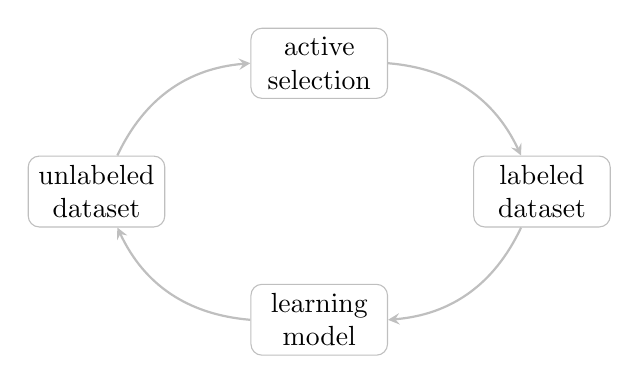
\begin{tikzpicture} [node distance = 4cm, on grid, auto]
 
\node (q0) [draw,lightgray, rounded corners, text width=1.5cm,yshift=-1.2cm, align =center] {\textcolor{black}{unlabeled \\dataset}};
\node (q1) [draw,lightgray, text width=1.5cm, rounded corners,above right = of q0,  yshift=-1.2cm,align =center] {\textcolor{black}{active \\selection}};
\node (q2) [draw,lightgray,rounded corners, text width=1.5cm, below right = of q1,yshift=1.2cm,align =center] {\textcolor{black}{labeled \\dataset}};
\node (q3) [draw,lightgray,rounded corners, text width=1.5cm, below left = of q2,yshift=1.2cm,align =center] {\textcolor{black}{learning \\model}};
 
\path [-stealth, thick]
    (q0) edge [lightgray, bend left]  (q1)
    (q1) edge [lightgray,bend left]  (q2)
    (q3) edge [lightgray,bend left]  (q0)
    (q2) edge [lightgray,bend left]  (q3);
\end{tikzpicture}
\caption{Active learning core structure. At each iteration a novel point is actively selected from the unlabeled set of data and the corresponding label is requested. Based on the received information, the model is modified.} \label{al}
\end{figure}